\begin{frame}{Chef}

    \begin{columns}

		\begin{column}{.4\hsize}
			\begin{figure}
				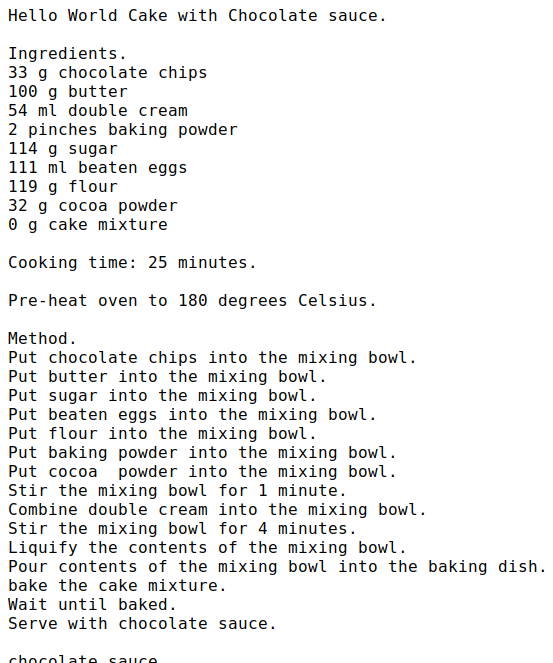
\includegraphics[height=6cm]{figures/chef1.png}
				\caption*{\footnotesize Przepis na ciasto HelloWorld {\color{blue} \hyperlink{frame:przypisy}{(6)}}}
			\end{figure}
		\end{column}

		\begin{column}{.6\hsize}
            \hspace{0.5cm}
			\begin{itemize}
				\myitem David Morgan-Mar, 2003
				\myitem Kod źródłowy przypomina przepis kulinarny
				\myitem Niepisanym wyzwaniem jest pisanie programów z których da się też przygotować posiłek
			\end{itemize}
            % \begin{figure}
            %     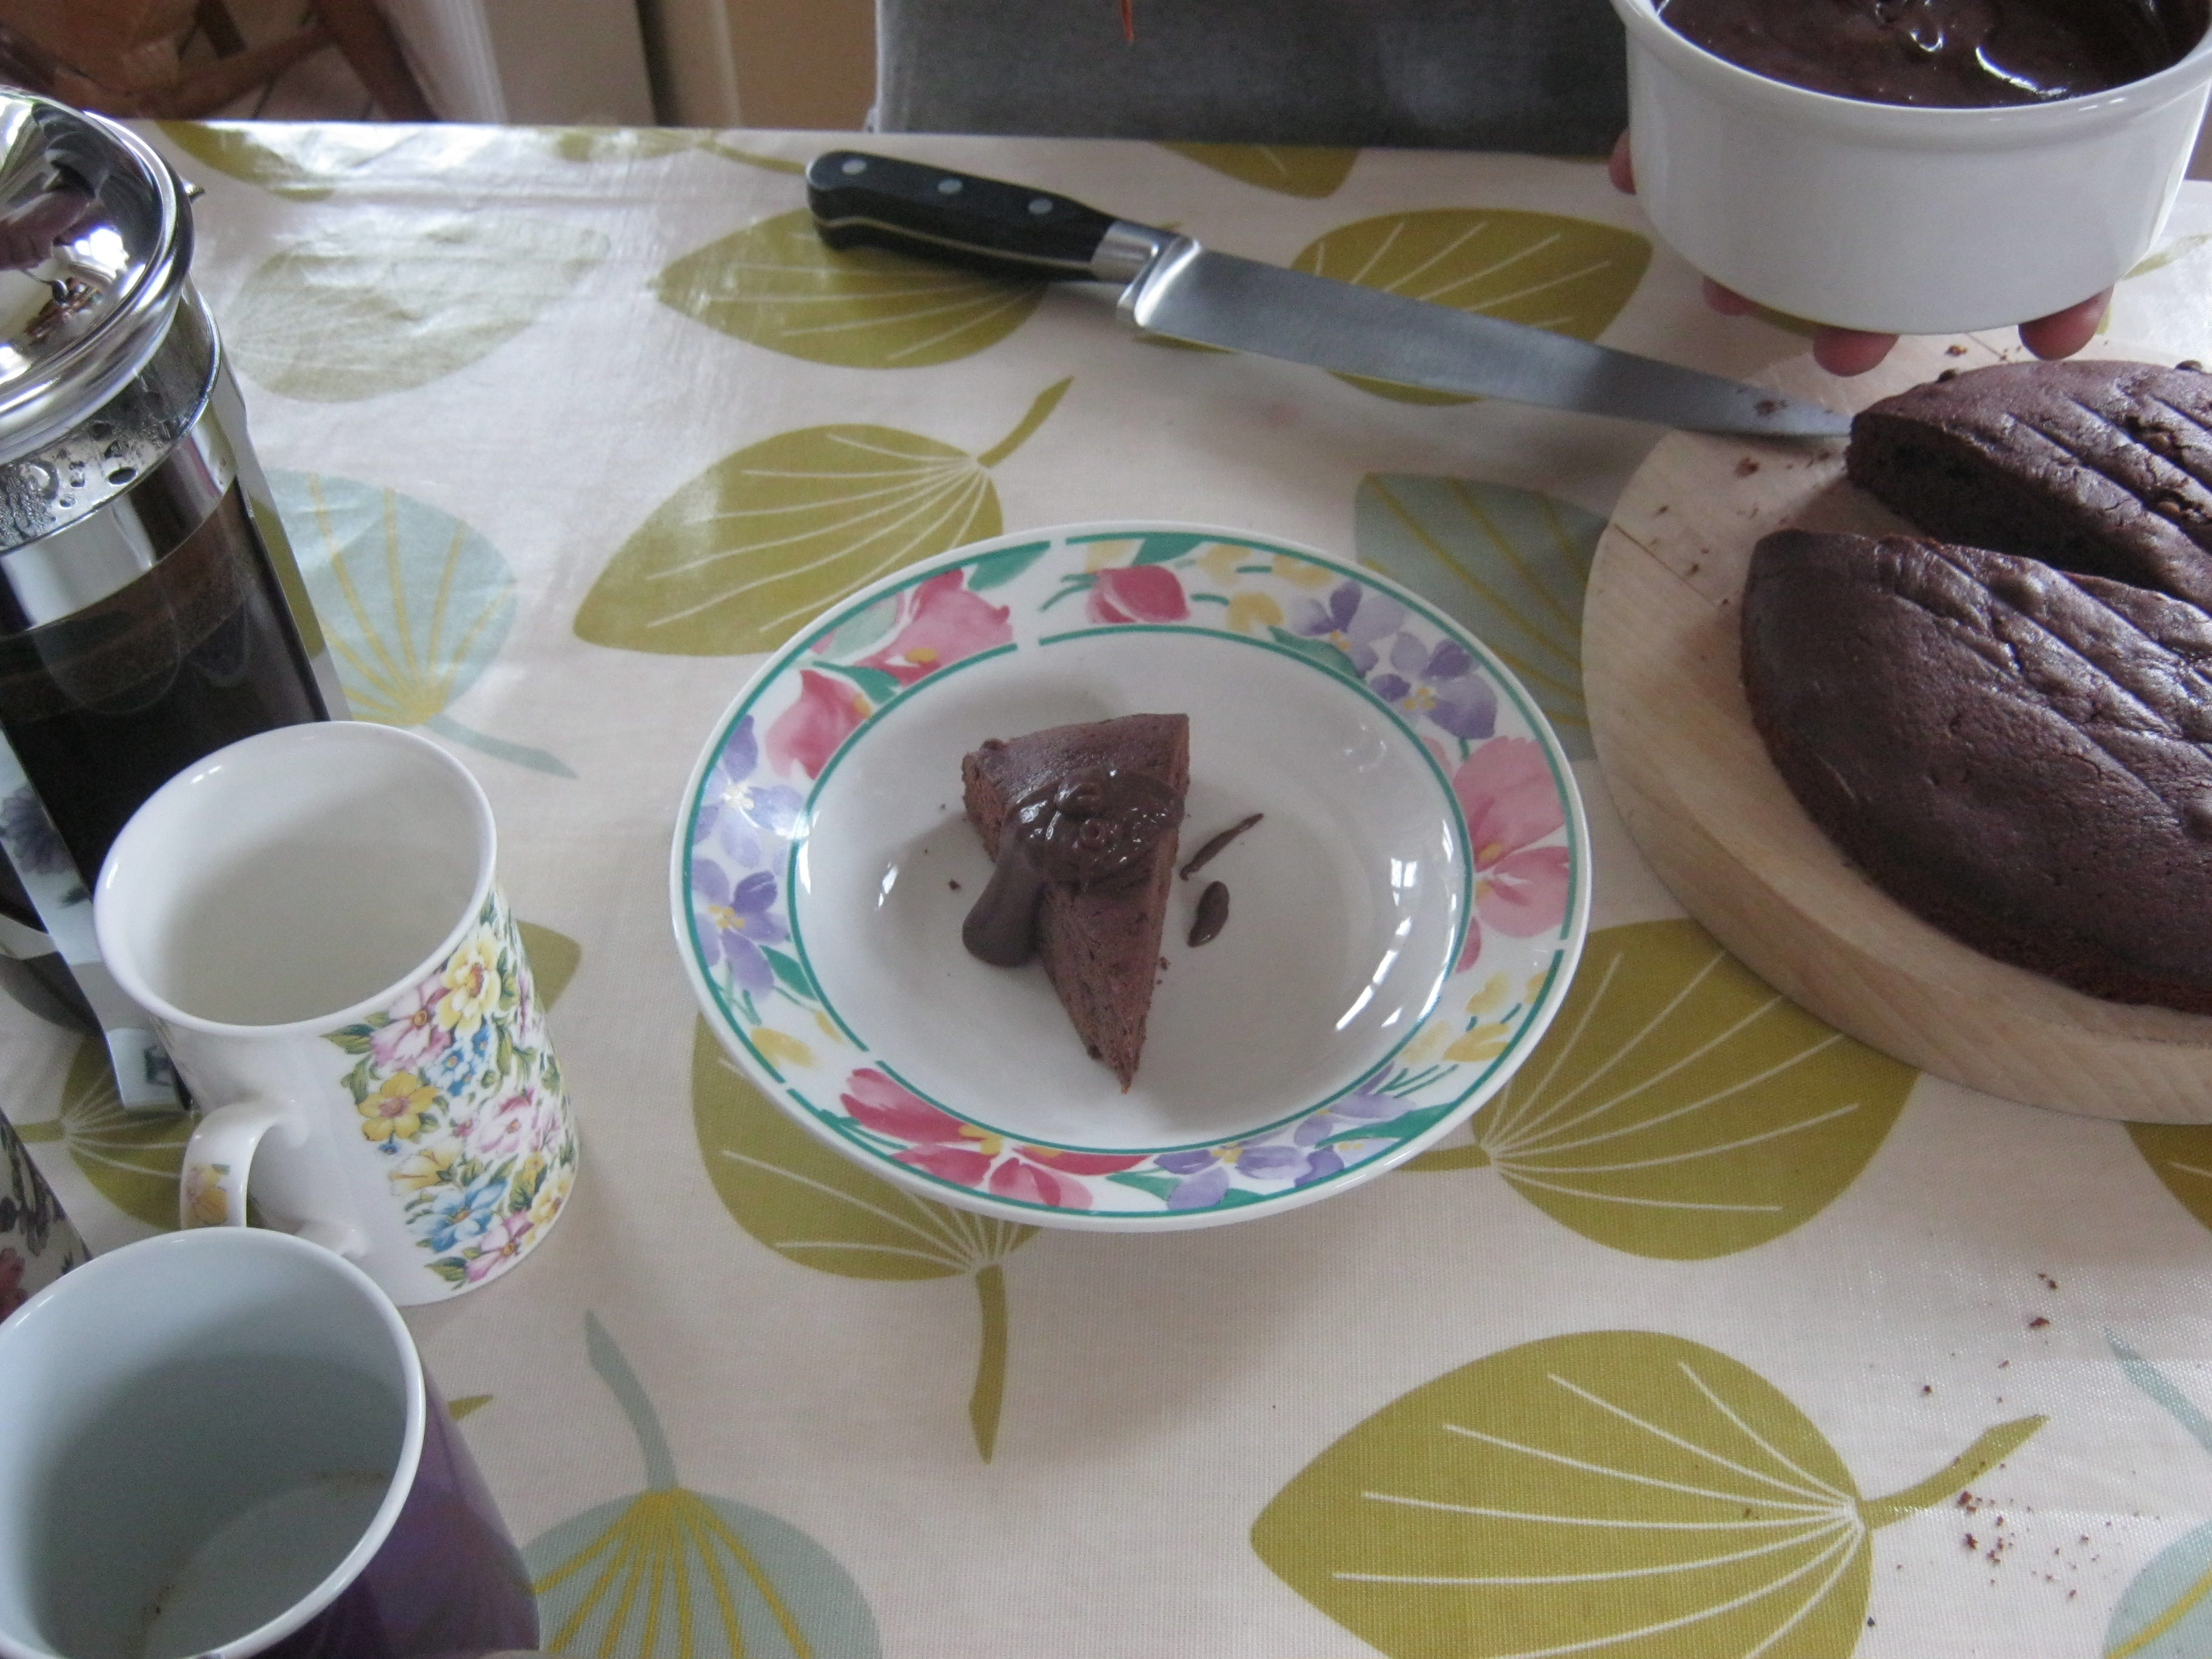
\includegraphics[width=4.5cm]{figures/chef_cake.jpg}
            %     \caption{\scriptsize Ciasto ,,HelloWorld'' autorstwa Mike Worth}
            % \end{figure}
		\end{column}

	\end{columns}

\end{frame}
